%!TEX root = Thesis.tex

\chapter{Catalytic Activity of Palladium Dioxygen Complexes}
\chaptermark{Catalysis}
\label{ch:catalysis}

Palladium catalysed coupling reactions are highly versatile and widely used tools for carbon-carbon bond formation.  Indeed the 2010 nobel prize in chemistry was awarded to Heck, Negishi and Suzuki for their work on ``palladium-catalyzed cross couplings in organic synthesis.''  However, all of these are traditional coupling reactions combining a nucleophile and an electrophile.  Much less studied are the couplings of two electrophiles (reductive coupling) or two nucleophiles (oxidative coupling).

\begin{scheme}[h]
\begin{center}
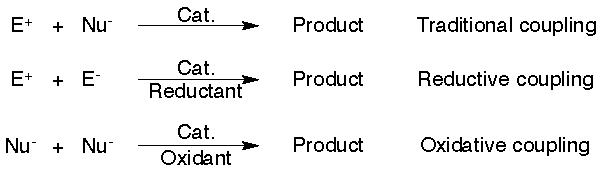
\includegraphics{../Schemes/Couplingreactions.pdf}
\caption[Types of coupling reactions]{Types of coupling reactions.}
\label{Couplingreactions}
\end{center}
\end{scheme}

Nucleophiles are some of the most naturally abundant and commonly used chemicals applied in organic synthesis.  Hence the direct coupling of two nucleophiles is a sought after methodology and has become the subject of much research recently.  In order to combine two nucleophiles an additional oxidant is needed.  A large body of research has focussed on the use of external oxidants such as TBHP, V2O5, H2O2 and benzoquinone, typically with high catalyst loadings of 5 - 10 mol\%.  An alternative oxidant is atmospheric oxygen and these reactions are generally also successful when performed under an oxygen atmosphere.  However, this leads to additional safety concerns.  More recently the use of palladium dioxygen complexes has allowed the oxidative coupling of aryl boronic acids in the air.  


